\documentclass[final]{beamer}
\usepackage[orientation=landscape,size=a0,scale=0.85]{beamerposter}
\usepackage{graphicx}
\usepackage{booktabs}
\usepackage{amsmath,amssymb,amsfonts}
\usepackage{multirow}
\usepackage{tikz}
\usetikzlibrary{arrows.meta,shapes.geometric,positioning}
\usepackage{tcolorbox}
\usepackage{xcolor}
\usepackage{colortbl}
\usepackage{array}
\usepackage{adjustbox}
\usepackage{enumitem}
\setlist[itemize]{leftmargin=12pt,itemsep=3pt,topsep=2pt,parsep=0pt}

% ---- Colors ----
\definecolor{FSUgarnet}{RGB}{120,47,64}
\definecolor{FSUgold}{RGB}{206,184,136}
\definecolor{accentblue}{RGB}{49,104,142}
\definecolor{accentgreen}{RGB}{40,150,100}
\definecolor{lightbg}{RGB}{248,248,252}
\definecolor{vlblue}{RGB}{228,238,250}
\definecolor{vlgreen}{RGB}{228,248,238}
\definecolor{lightyellow}{RGB}{255,250,230}
\definecolor{vlgarnet}{RGB}{248,236,239}

\usetheme{default}
\setbeamercolor{background canvas}{bg=lightbg}
\setbeamertemplate{navigation symbols}{}
\tcbuselibrary{skins}

\newtcolorbox{posterblock}[1]{
  colback=white, colframe=FSUgarnet, coltitle=white,
  fonttitle=\large\bfseries, title=#1,
  arc=3mm, boxrule=2pt,
  toptitle=4pt, bottomtitle=4pt,
  top=5pt, bottom=5pt, left=8pt, right=8pt,
  colbacktitle=FSUgarnet, enhanced
}
\newtcolorbox{methodbox}[1]{
  colback=white, colframe=accentblue, coltitle=white,
  fonttitle=\large\bfseries, title=#1,
  arc=3mm, boxrule=2pt,
  toptitle=4pt, bottomtitle=4pt,
  top=5pt, bottom=5pt, left=8pt, right=8pt,
  colbacktitle=accentblue, enhanced
}
\newtcolorbox{appblock}[1]{
  colback=white, colframe=accentgreen!80!black, coltitle=white,
  fonttitle=\large\bfseries, title=#1,
  arc=3mm, boxrule=2pt,
  toptitle=4pt, bottomtitle=4pt,
  top=5pt, bottom=5pt, left=8pt, right=8pt,
  colbacktitle=accentgreen!80!black, enhanced
}
\newtcolorbox{keybox}{
  colback=lightyellow, colframe=FSUgold!80!black,
  arc=2mm, boxrule=1.2pt,
  top=4pt, bottom=4pt, left=6pt, right=6pt,
}
\newtcolorbox{stagebox}[1]{
  colback=vlblue, colframe=accentblue!60,
  arc=2mm, boxrule=1pt,
  top=3pt, bottom=3pt, left=5pt, right=5pt,
  fonttitle=\normalsize\bfseries, title=#1, colbacktitle=accentblue!60, coltitle=white,
  toptitle=2pt, bottomtitle=2pt
}
\newtcolorbox{spatialbox}{
  colback=vlgarnet, colframe=FSUgarnet!50,
  arc=2mm, boxrule=1pt,
  top=3pt, bottom=3pt, left=5pt, right=5pt,
}
\newtcolorbox{findingbox}{
  colback=vlgreen, colframe=accentgreen!60,
  arc=2mm, boxrule=1pt,
  top=3pt, bottom=3pt, left=6pt, right=6pt,
}

\begin{document}
\begin{frame}[fragile]

% ====== HEADER ======
\begin{tcolorbox}[
  colback=FSUgarnet, colframe=FSUgarnet, arc=0mm, boxrule=0pt,
  top=8pt, bottom=5pt, left=30pt, right=30pt, width=\textwidth
]
\centering
{\color{FSUgold}\VeryHuge\bfseries Estimation of Cluster-Specific Causal Effects on Spatially Associated Survival Data Using SoftBART}\\[10pt]
{\color{white}\LARGE Durbadal Ghosh}\\[3pt]
{\color{FSUgold}\large Department of Statistics, Florida State University}\\[2pt]
{\color{white}\small Joint work with I.\ Bhattacharya, D.\ Sinha, and G.\ Rust}
\end{tcolorbox}

\vspace{5pt}

\begin{columns}[T]

% ==================== COLUMN 1 (35%): MOTIVATION ====================
\begin{column}{0.335\textwidth}

\begin{posterblock}{The Problem: Treatment Delay in Breast Cancer}

\begin{keybox}
\centering
\textbf{Does delaying breast cancer treatment ($>$90 days) \emph{cause} worse survival? And how does the effect vary across geographic regions?}
\end{keybox}

\vspace{4pt}

\begin{minipage}[t]{0.47\textwidth}
{\color{FSUgarnet}\textbf{Breast Cancer Facts}}
\begin{itemize}
\item Most diagnosed cancer in US women
\item 2nd leading cause of cancer death
\item \textbf{Treatment Delay (TD):} diagnosis $\to$ first treatment
\item TD $>$ 90 days $\Rightarrow$ worse 5-yr survival
\end{itemize}
\end{minipage}\hfill
\begin{minipage}[t]{0.50\textwidth}
{\color{FSUgarnet}\textbf{Florida Cancer Registry (FCR)}}
\begin{itemize}
\item $N = 68{,}009$ patients, $K = 67$ counties
\item 41.3\% right-censored
\item $Z\!=\!1$ (TD $\leq 90$ d) vs.\ $Z\!=\!0$ (TD $> 90$ d)
\item Confounders: Age, HR status, Tumor Grade, Biopsy Delay
\end{itemize}
\end{minipage}
\end{posterblock}

\vspace{4pt}

\begin{posterblock}{Key Challenges}
\begin{minipage}[t]{0.47\textwidth}
{\color{FSUgarnet}\textbf{Data}}
\begin{itemize}
\item[$\triangleright$] \textbf{Spatial dependence} --- neighboring counties share profiles
\item[$\triangleright$] \textbf{Right-censoring} (41.3\%)
\item[$\triangleright$] \textbf{Confounded} treatment (not random)
\item[$\triangleright$] \textbf{Clustered} --- patients within counties
\end{itemize}
\end{minipage}\hfill
\begin{minipage}[t]{0.50\textwidth}
{\color{FSUgarnet}\textbf{Modeling}}
\begin{itemize}
\item[$\triangleright$] \textbf{Non-linear} treatment--confounder--outcome links
\item[$\triangleright$] \textbf{Unmeasured} county-level confounding
\item[$\triangleright$] Need \textbf{county-} \& \textbf{patient-specific} effects
\item[$\triangleright$] No method does spatial $+$ nonparametric $+$ survival
\end{itemize}
\end{minipage}
\end{posterblock}

\vspace{4pt}

\begin{posterblock}{Goal \& Causal Estimands}

{\color{FSUgarnet}\textbf{Counterfactual survival:}} $S^{(z)}_{ij}(t\mid\mathbf{x}_{ij}) = P\bigl(T_{ij}(z)\geq t \mid \mathbf{x}_{ij}, \text{County}=i\bigr)$

\vspace{4pt}
\begin{keybox}
\centering
\textbf{Patient-level --- CERM} (restricted mean gain over $(0,t^*)$):\\[2pt]
$\text{CERM}_{ij}(t^*) = \mathbb{E}\bigl[\{T_{ij}(1)\wedge t^*\} - \{T_{ij}(0)\wedge t^*\} \mid \mathbf{x}_{ij},\, i\bigr]$
\end{keybox}

\vspace{4pt}
{\color{FSUgarnet}\textbf{Multi-resolution aggregation:}}
\begin{itemize}
\item \textbf{County:}\; $\text{ACERM}_i(t^*) = \frac{1}{n_i}\sum_{j}\text{CERM}_{ij}(t^*)$\; (also for treated/untreated: ACERMT, ACERMU)
\item \textbf{State:}\; $\text{RATE}(t^*) = \frac{1}{N}\sum_{i,j}\text{CERM}_{ij}(t^*)$\; (RATT, RATU by group)
\item \textbf{Survival-prob effect:}\; $\text{SPTE}_i(t) = S^{(1)}_i(t) - S^{(0)}_i(t)$
\end{itemize}

\vspace{4pt}
{\color{FSUgarnet}\textbf{Identifiability under:}} SUTVA, Consistency, Unconfoundedness, Positivity, Non-informative censoring.

\vspace{5pt}
\centering
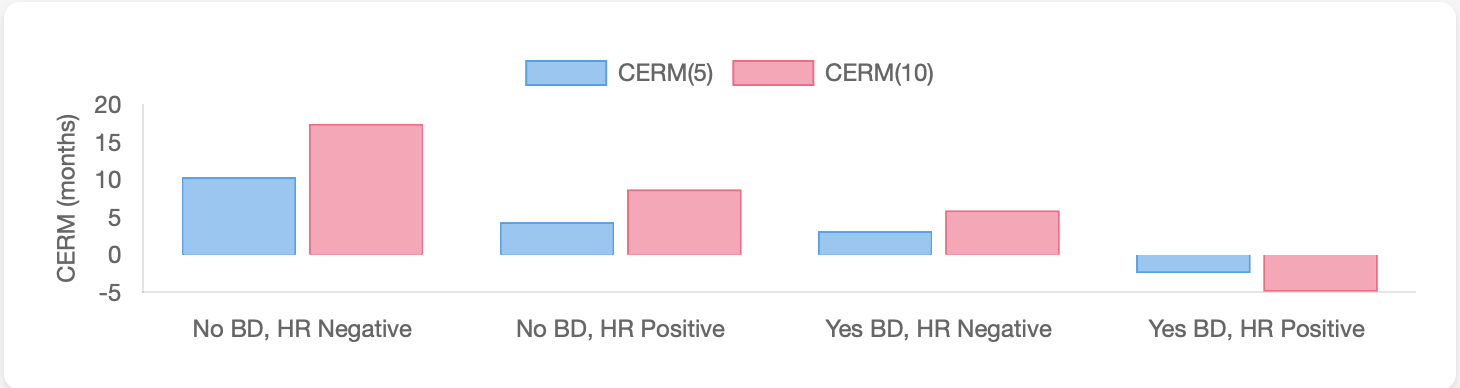
\includegraphics[width=0.92\textwidth]{BD_HR.png}\\
\raggedright
\vspace{1pt}
{\scriptsize Heterogeneous CERM (months) by Biopsy Delay \& HR status --- effects differ sharply across subgroups, motivating a \emph{flexible} model.}
\end{posterblock}

\end{column}

% ==================== COLUMN 2 (37%): METHOD + SIM ====================
\begin{column}{0.355\textwidth}

\begin{methodbox}{Proposed Method: PS-LND (Soft BART $+$ DAGAR)}

\centering
{\small\textbf{Data} $(y_{ij},\delta_{ij},z_{ij},\mathbf{x}_{ij})$\; $\Longrightarrow$\; {\color{accentblue}\textbf{Stage 1:}} estimate PS $\hat{e}_{ij}$\; $\Longrightarrow$\; {\color{accentblue}\textbf{Stage 2:}} survival outcome\; $\Longrightarrow$\; {\color{accentgreen}\textbf{causal effects}}}
\raggedright

\vspace{3pt}
\begin{stagebox}{Stage 1 --- Propensity Score (Spatial Probit-SBART)}
\vspace{-3pt}
$$P(Z_{ij}=1\mid \mathbf{x}_{ij}, V_i) = \Phi\!\bigl(\underbrace{b(\mathbf{x}_{ij})}_{\text{SBART}} + \underbrace{V_i}_{\text{DAGAR}}\bigr),\qquad \hat{e}_{ij} = E[\,\Phi\{b(\mathbf{x}_{ij}) + V_i\}\mid\mathcal{D}_1\,]$$
\vspace{-7pt}
\begin{itemize}
\item $b(\cdot)$: unknown function with Soft BART prior;\; $\mathbf{V}\sim N(\mathbf{0},\tau_v^{-1}\mathbf{Q}(\rho_v)^{-1})$ captures \textbf{unmeasured spatial confounding}
\end{itemize}
\end{stagebox}

\vspace{3pt}
\begin{stagebox}{Stage 2 --- Outcome (Log-Normal AFT with BCF structure)}
\vspace{-3pt}
$$\log T_{ij} \sim N\!\Bigl(\underbrace{\mu(\mathbf{x}_{ij}, \hat{e}_{ij})}_{\text{prognostic SBART}} + \underbrace{\tau(\mathbf{x}_{ij})}_{\text{treatment SBART}}\!\cdot Z_{ij} + \underbrace{W_i}_{\text{county DAGAR}},\;\; \sigma^2\Bigr)$$
\vspace{-7pt}
\begin{itemize}
\item Separate prognostic $\mu$ \& treatment $\tau$ surfaces handle \textbf{targeted selection}; $\hat{e}_{ij}$ enters as a confounder
\item $\mathbf{W}\sim N(\mathbf{0},\tau_w^{-1}\mathbf{Q}(\rho_w)^{-1})$: county random effects; right-censoring via data augmentation
\end{itemize}
\end{stagebox}

\vspace{3pt}
\begin{spatialbox}
{\color{FSUgarnet}\textbf{DAGAR spatial prior --- interpretable smoothing.}} For county $i$ with preceding neighbors $\mathcal{N}(i)$:
\vspace{-3pt}
$$W_i \mid W_{\mathcal{N}(i)} \sim N\!\Bigl(\tfrac{\rho_w}{1+(n_i-1)\rho_w^2}\!\!\sum_{j\in\mathcal{N}(i)}\!\! W_j,\;\; \tfrac{1+(n_i-1)\rho_w^2}{\tau_w(1-\rho_w^2)}\Bigr)$$
\vspace{-7pt}
\begin{itemize}
\item $\rho_w\!\to\!0$: counties independent;\; $\rho_w\!\to\!1$: strong neighbor smoothing
\item Pairwise correlations stay $\approx\rho_w$ --- genuine ``borrowing of strength''
\end{itemize}
\end{spatialbox}
\end{methodbox}

\vspace{4pt}

\begin{methodbox}{Why PS-LND Wins --- Key Novelties}
\begin{minipage}[t]{0.49\textwidth}
\begin{itemize}[itemsep=4pt]
\item[\color{accentgreen}\Large$\checkmark$] \textbf{Flexible \& nonparametric:} Soft BART's \emph{smooth} sigmoid trees fit nonlinear effects with \emph{no} pre-specified interactions
\item[\color{accentgreen}\Large$\checkmark$] \textbf{Interpretable spatial (DAGAR):} proper, sparse, positive-definite precision; $\rho_w\!\in\!(0,1)$; scalable
\item[\color{accentgreen}\Large$\checkmark$] \textbf{Doubly robust:} consistent if \emph{either} PS or outcome model is correct
\end{itemize}
\end{minipage}\hfill
\begin{minipage}[t]{0.49\textwidth}
\begin{itemize}[itemsep=4pt]
\item[\color{accentgreen}\Large$\checkmark$] \textbf{No feedback:} two-stage design isolates PS from a misspecified outcome; efficient
\item[\color{accentgreen}\Large$\checkmark$] \textbf{Targeted selection (BCF):} splits prognostic vs.\ treatment effect for clean heterogeneity
\item[\color{accentgreen}\Large$\checkmark$] \textbf{County-specific \& multi-level:} full posterior for patient, county \& state effects
\end{itemize}
\end{minipage}
\end{methodbox}

\vspace{4pt}

\begin{methodbox}{Simulation: Verifying the Method}
$K\!=\!35$ clusters on a $5\!\times\!7$ grid, $N\!=\!1750$, 5 confounders, 150 replications. Method stress-tested under three regimes:

\vspace{3pt}
\begin{adjustbox}{max width=\textwidth}
\renewcommand{\arraystretch}{1.15}
\footnotesize
\begin{tabular}{p{1.9cm} p{4.7cm} p{6.5cm}}
\toprule
\textbf{Scenario} & \textbf{What it tests} & \textbf{Data-generating truth} \\
\midrule
\textbf{1. Ideal} & Correct specification & Log-Normal $+$ DAGAR effects ($\rho_w\!=\!0.7$); nonlinear main effects $+$ treatment interactions \\
\textbf{2. Misspecified} & Robustness to model error & Adds covariate $\times$ random-effect interactions $g(\mathbf{x},z,w)$ omitted by fitted model \\
\textbf{3. Stress test} & Distribution violation $+$ heavy censoring & Weibull (not log-Normal), 50\% censoring, \emph{strong} confounding \\
\bottomrule
\end{tabular}
\end{adjustbox}

\vspace{4pt}
\begin{adjustbox}{max width=\textwidth}
\renewcommand{\arraystretch}{1.1}
\small
\begin{tabular}{ll >{\bfseries}c c c c}
\toprule
\textbf{Scenario} & \textbf{Metric} & \textbf{PS-LND} & riAFTBART & PSW-Fr. & IPW \\
\midrule
\textbf{1. Ideal} & Cov / MAE & \cellcolor{vlgreen}0.93--0.97 / 0.01 & 0.46--0.95 / 0.08--0.58 & 0.54--0.97 / 0.08--0.50 & 0.38--0.52 / 0.06 \\
\textbf{2. Misspec.} & Cov / MAE & \cellcolor{vlgreen}0.92--0.95 / 0.01 & 0.77--0.89 / 0.20--0.79 & 0.64--0.89 / 0.21--0.63 & 0.42--0.53 / 0.06 \\
\textbf{3. Stress} & Cov / MAE & \cellcolor{vlgreen}0.87--0.90 / 0.03 & 0.55--0.68 / 0.24--0.66 & 0.76--0.82 / 0.08--0.21 & 0.42--0.47 / 0.53 \\
\bottomrule
\end{tabular}
\end{adjustbox}

\vspace{3pt}
\begin{findingbox}
\centering
\textbf{PS-LND attains near-nominal coverage \& the lowest MAE in every regime} --- the only method robust to misspecification \emph{and} distributional violation.
\end{findingbox}
\end{methodbox}

\end{column}

% ==================== COLUMN 3 (28%): APPLICATION ====================
\begin{column}{0.28\textwidth}

\begin{appblock}{Application: Florida Cancer Registry --- WA-Distant Stratum}

{\color{accentgreen!80!black}\textbf{Patient-Level Effects (Broward County)}}\\[2pt]
\centering
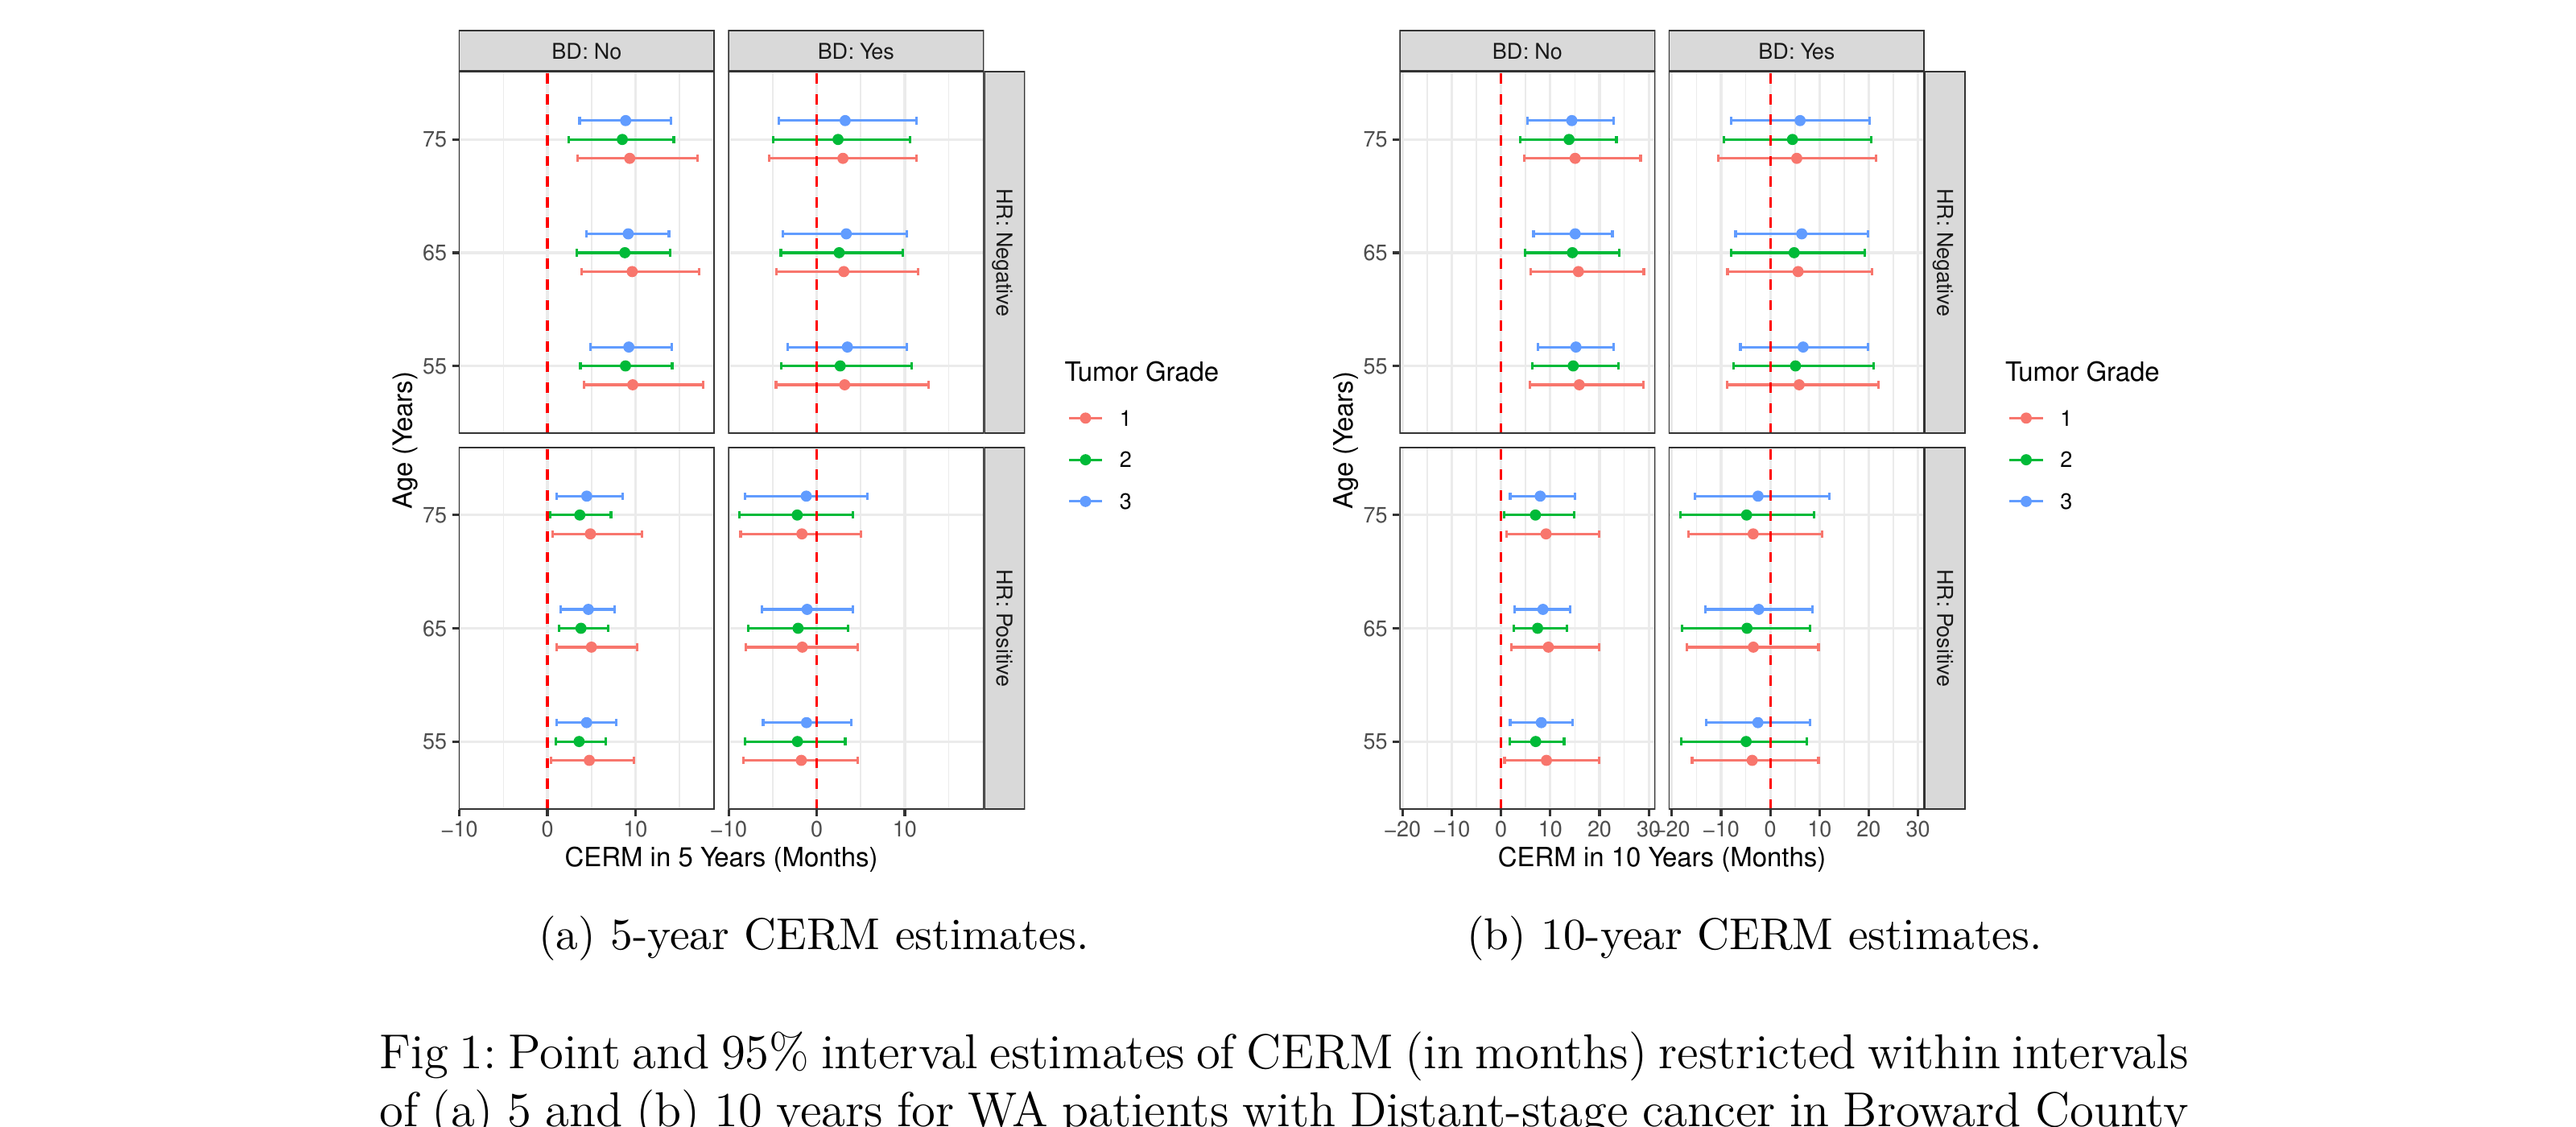
\includegraphics[width=0.97\textwidth]{poster_figs/cerm_plot.png}\\
\raggedright
\vspace{1pt}
{\scriptsize $\widehat{\text{CERM}}$ (months) at 5 \& 10 yr by Age, BD, HR, Tumor Grade ($n\!=\!183$)}

\vspace{3pt}
\begin{itemize}
\item HR$-$, no BD: \textbf{13.8--15.9 mo.} gain (10 yr)
\item HR$+$, no BD: \textbf{6.9--9.6 mo.} gain
\item With biopsy delay: no significant effect (CI $\ni$ 0)
\end{itemize}

\vspace{4pt}
{\color{accentgreen!80!black}\textbf{County-Level Spatial Patterns}}\\[2pt]
\centering
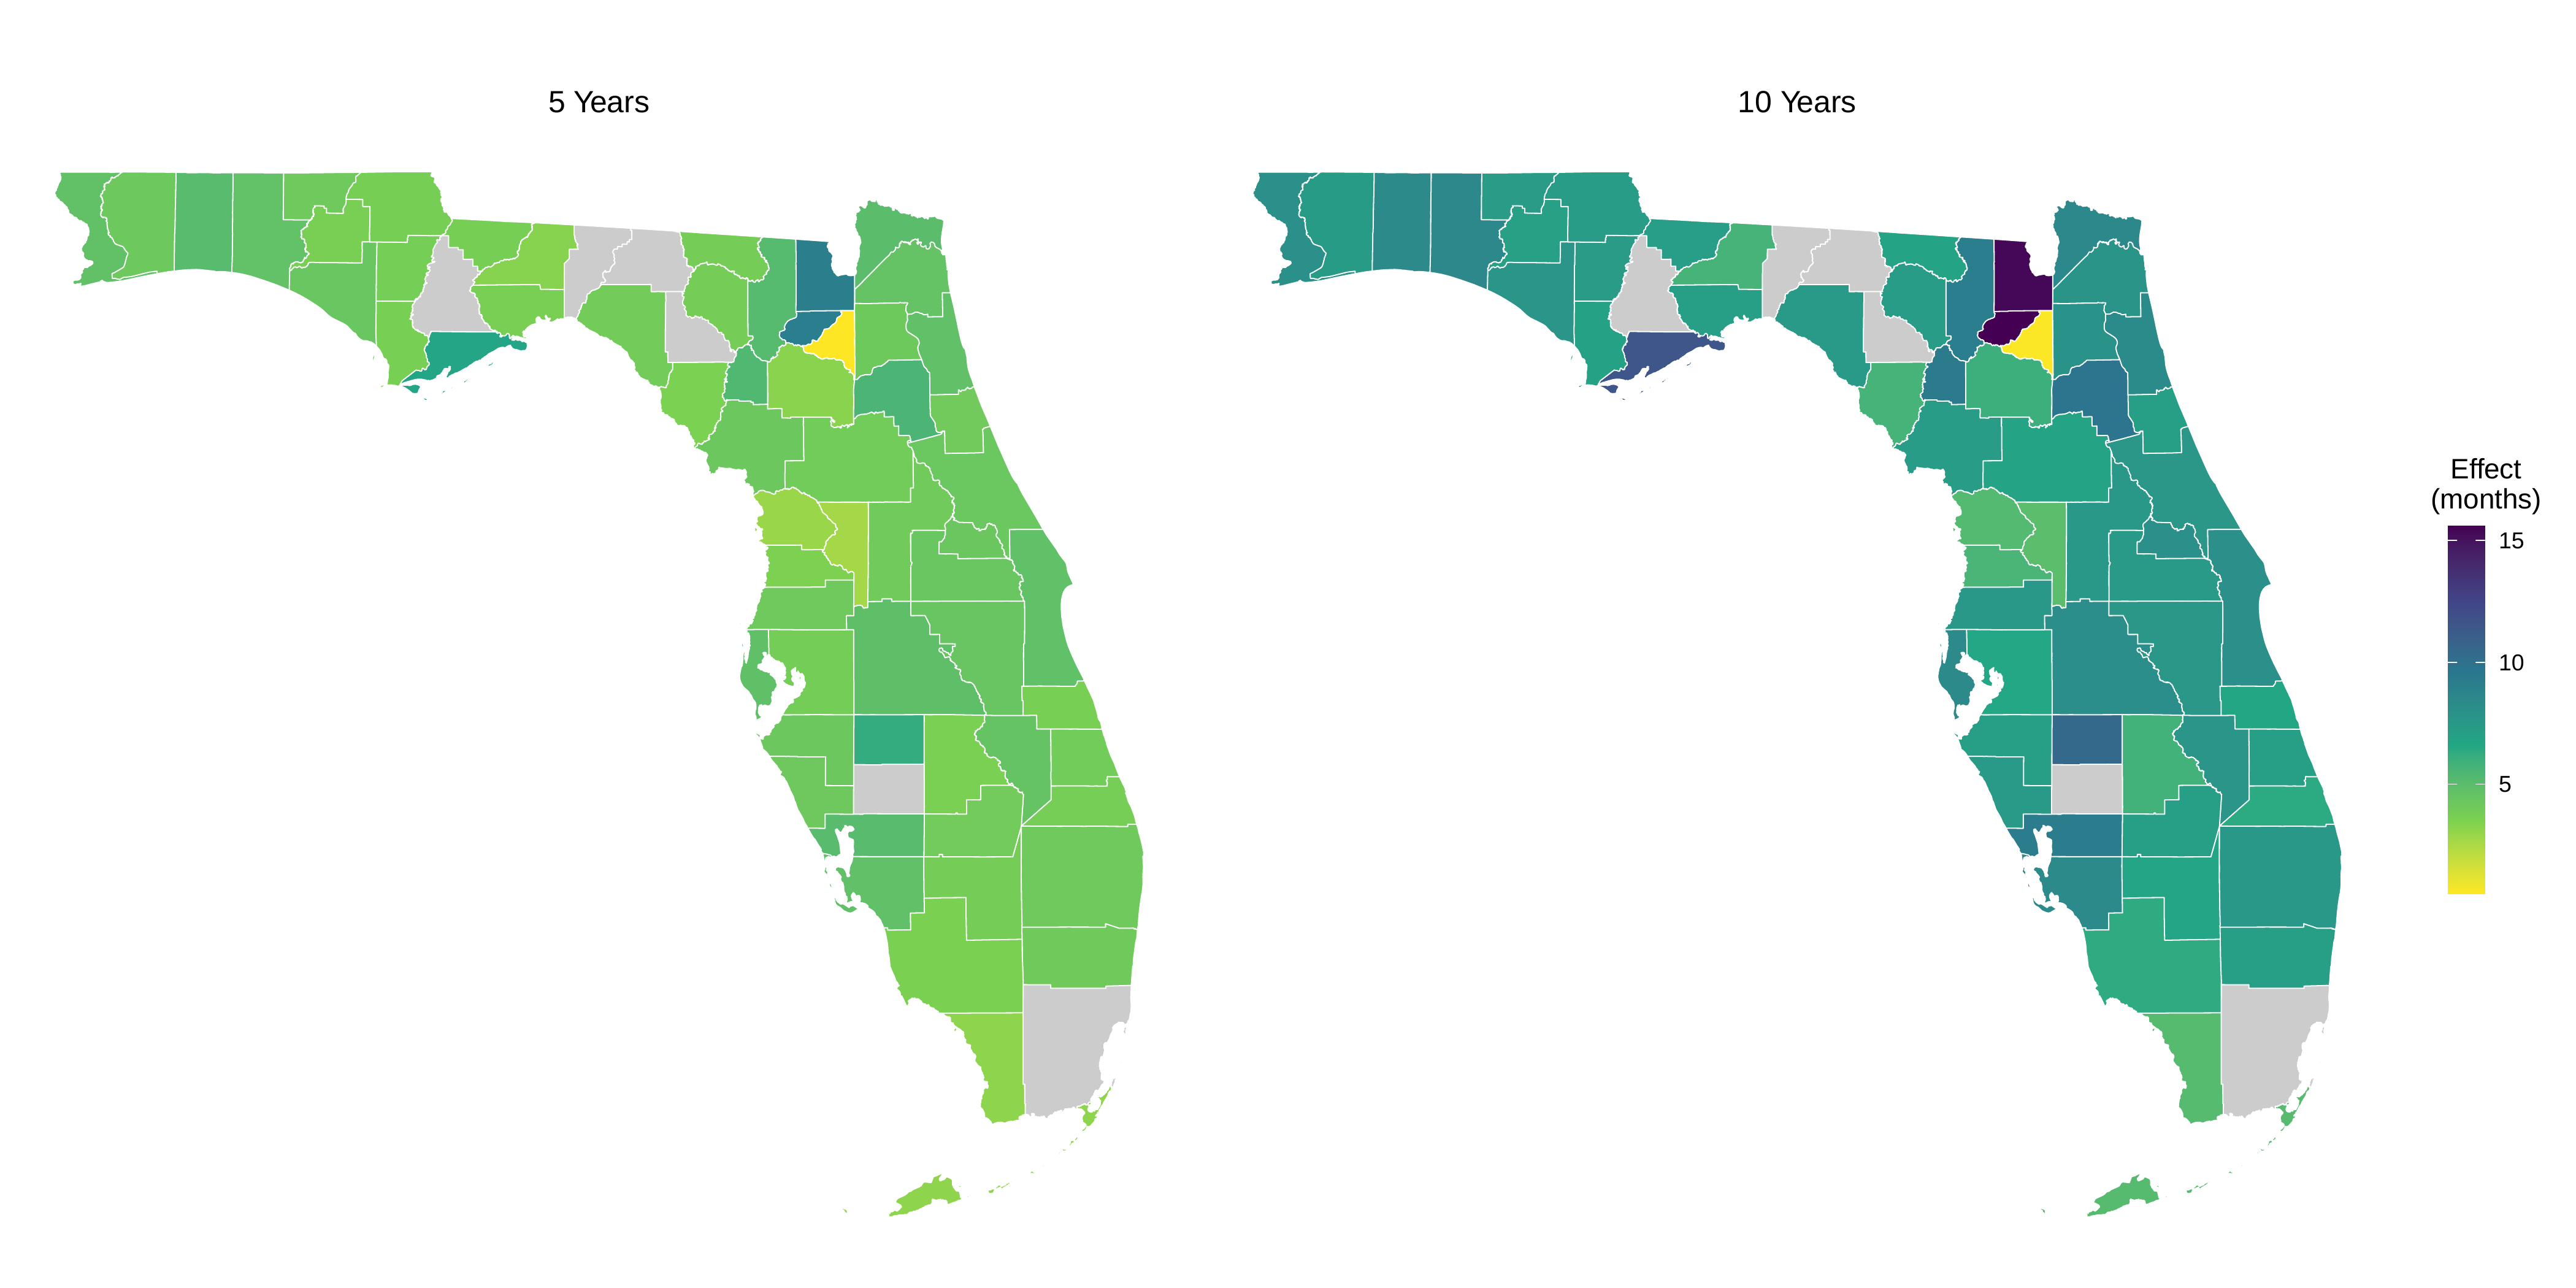
\includegraphics[width=0.97\textwidth]{poster_figs/crate-1.png}\\
\raggedright
\vspace{1pt}
{\scriptsize $\widehat{\text{ACERM}}_i$ at 5 (left) \& 10 (right) yr. Yellow $=0$ mo $\to$ dark $=15{+}$ mo; gray $=$ no data}

\vspace{3pt}
\begin{itemize}
\item Highest: Union ($>$15 mo.), Baker ($>$13 mo.)
\item Near-zero: Bradford (CI $\ni$ 0)
\item Clear \textbf{spatial clustering} of treatment effects
\end{itemize}

\vspace{4pt}
{\color{accentgreen!80!black}\textbf{State-Wide Treatment Effects}}\\[2pt]
\centering
\begin{adjustbox}{max width=0.97\textwidth}
\renewcommand{\arraystretch}{1.1}
\begin{tabular}{lccc}
\toprule
\textbf{Estimand} & $\boldsymbol{N}$ & \textbf{Est.\ (mo.)} & \textbf{95\% CI} \\
\midrule
\rowcolor{vlgreen} RATE (10 yr) & 1994 & \textbf{7.62} & (4.42, 10.86) \\
RATT (10 yr) & 687 & 6.74 & (3.09, 10.08) \\
\rowcolor{vlgreen} RATU (10 yr) & 1307 & \textbf{8.09} & (4.60, 11.42) \\
RATE (5 yr) & 1994 & 4.43 & (2.56, 6.23) \\
\bottomrule
\end{tabular}
\end{adjustbox}

\raggedright
\vspace{3pt}
\begin{itemize}
\item \textbf{No CI contains zero} $\Rightarrow$ strong evidence
\item \textbf{RATU $>$ RATT}: long-TD patients gain the most
\item Benefits persist beyond 5 years
\end{itemize}

\vspace{4pt}
\centering
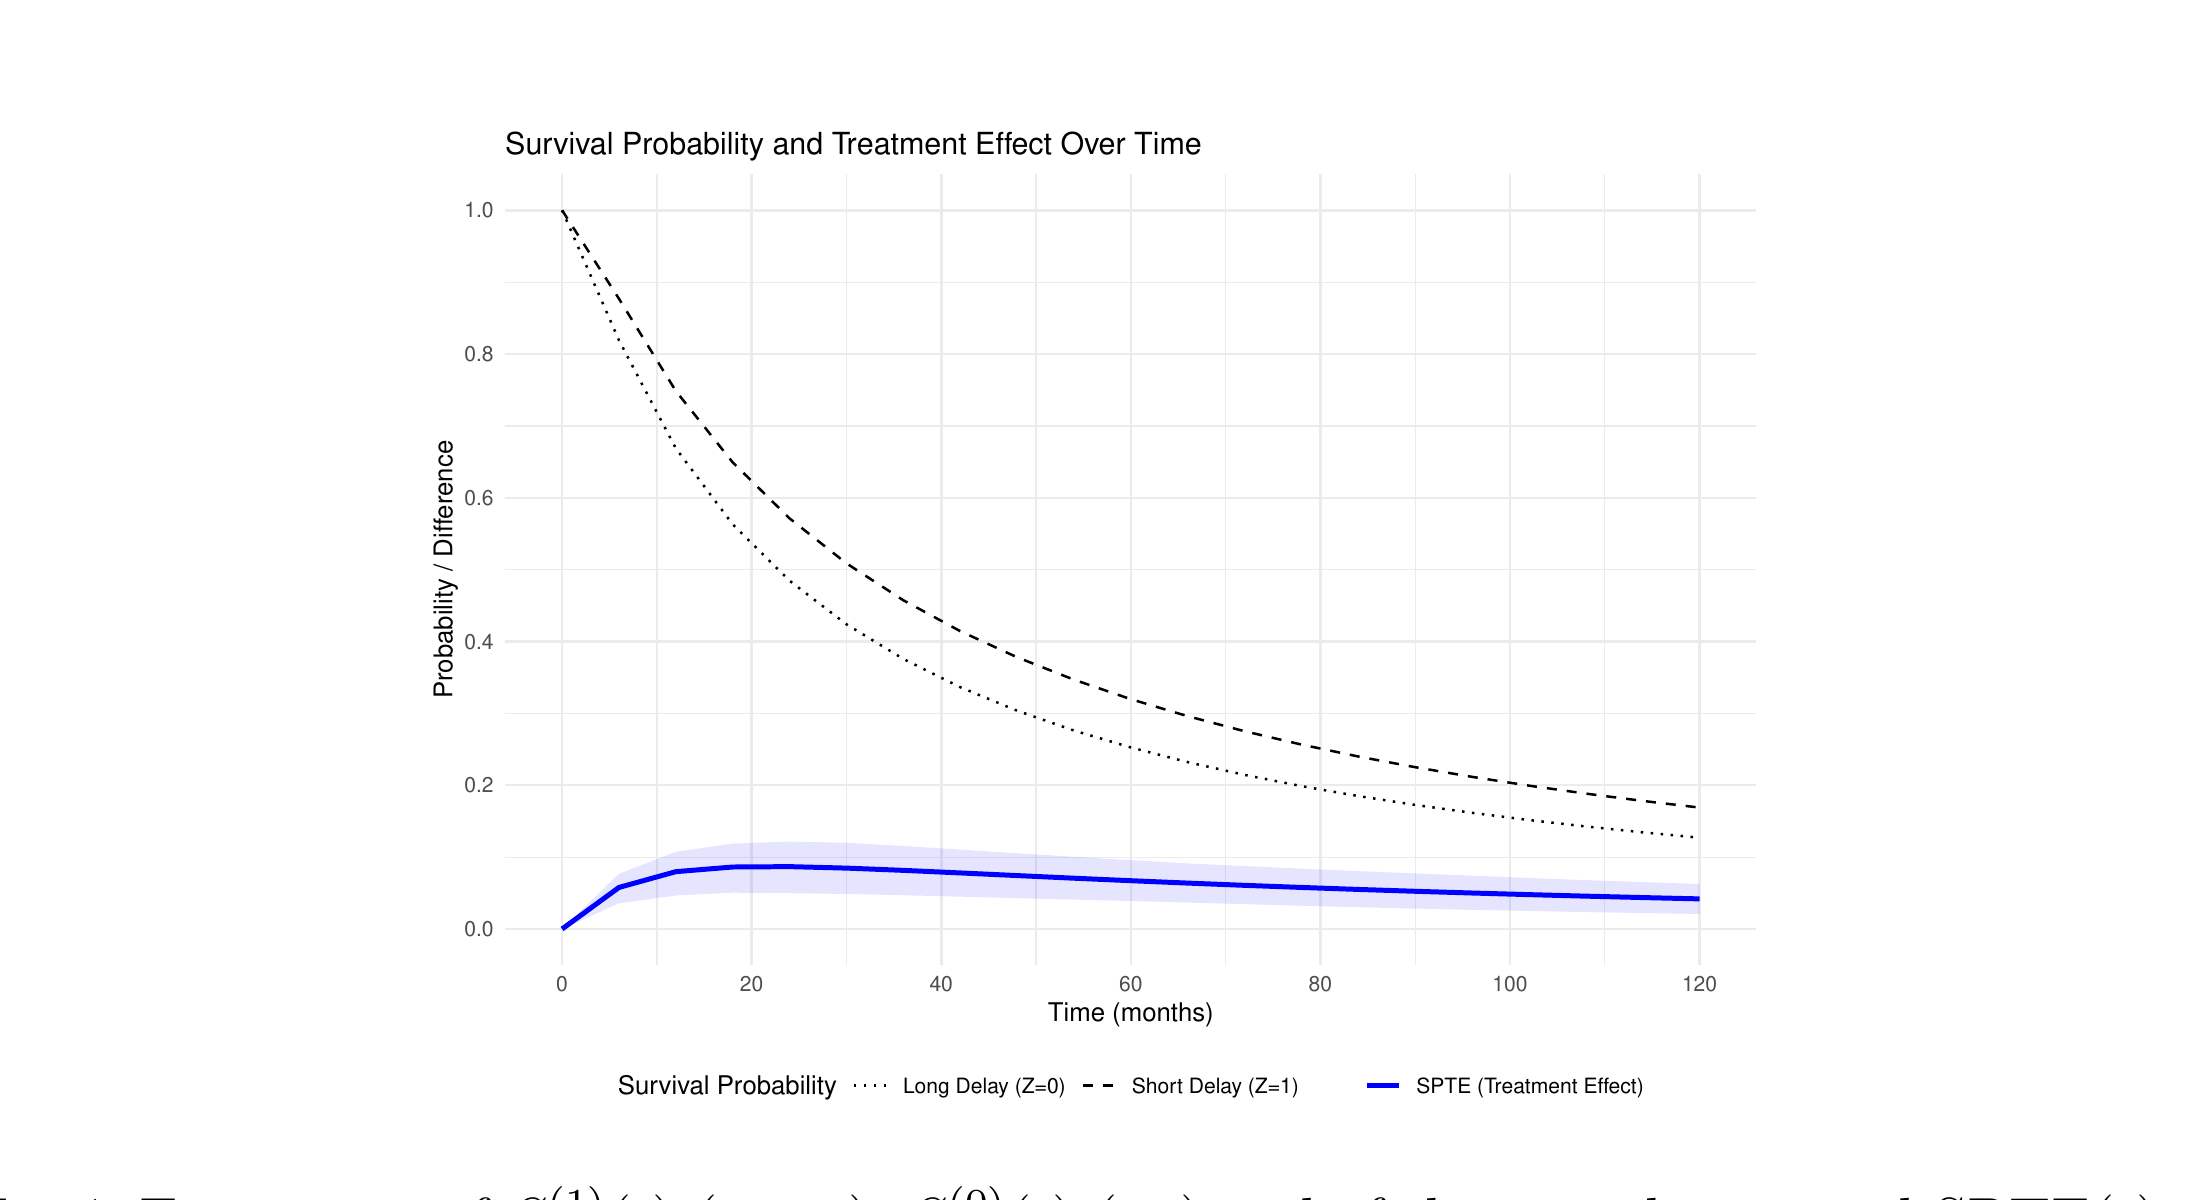
\includegraphics[width=0.82\textwidth]{poster_figs/spte_plot.png}\\
\raggedright
\vspace{1pt}
{\scriptsize $\widehat{\text{SPTE}}(t)$: peak \textbf{11\%} survival-probability gain at $t\!=\!2.2$ yr; CI $>0$ throughout}

\vspace{4pt}
\begin{keybox}
\centering
{\large\textbf{Policy Takeaway}}\\[2pt]
\begin{itemize}[itemsep=3pt]
\item Short TD $\Rightarrow$ \textbf{7.6 mo.} average survival gain statewide
\item Priority: \textbf{HR$-$ patients without biopsy delay}
\item Target \textbf{rural northern counties} for patient-navigation programs
\end{itemize}
\end{keybox}

\end{appblock}

\end{column}

\end{columns}

% ====== FOOTER ======
\vspace{3pt}
\begin{tcolorbox}[
  colback=FSUgarnet, colframe=FSUgarnet, arc=0mm, boxrule=0pt,
  left=30pt, right=30pt, top=4pt, bottom=4pt
]
{\color{white}\small
\textbf{Contact:} dg20ea@fsu.edu
\hfill
\textbf{Code:} \texttt{github.com/indrabati646/PS-LND-DAGAR}
\hfill
\textbf{Funding:} NIH R03CA205018-01, R21DE034124-01A1; NSF 2413549
\hfill
\textbf{Coauthors:} I.\ Bhattacharya, D.\ Sinha, G.\ Rust (FSU)
}
\end{tcolorbox}

\end{frame}
\end{document}
